%%%%%%%%%%%%%%%%%%%%%%%%%%%%%%%%%%%%%%%%%
% Short Sectioned Assignment
% LaTeX Template
% Version 1.0 (5/5/12)
%
% This template has been downloaded from:
% http://www.LaTeXTemplates.com
%
% Original author:
% Frits Wenneker (http://www.howtotex.com)
%
% License:
% CC BY-NC-SA 3.0 (http://creativecommons.org/licenses/by-nc-sa/3.0/)
%
%%%%%%%%%%%%%%%%%%%%%%%%%%%%%%%%%%%%%%%%%

%----------------------------------------------------------------------------------------
%	PACKAGES AND OTHER DOCUMENT CONFIGURATIONS
%----------------------------------------------------------------------------------------

\documentclass[paper=a4, fontsize=11pt]{scrartcl} % A4 paper and 11pt font size

\usepackage{graphicx}
\usepackage{xcolor}
\usepackage{listings}

\definecolor{grey}{rgb}{0.9,0.9,0.9}
\lstset{basicstyle=\ttfamily,
  showstringspaces=false,
  backgroundcolor=\color{grey},
  commentstyle=\color{red},
  keywordstyle=\color{blue}
}
\usepackage[hang, small,labelfont=bf,up,textfont=it,up]{caption} % Custom captions under/above floats in tables or figures
\usepackage{float} % Required for tables and figures in the multi-column environment - they need to be placed in specific locations with the [H] (e.g. \begin{table}[H])

\usepackage[T1]{fontenc} % Use 8-bit encoding that has 256 glyphs
%\usepackage{fourier} % Use the Adobe Utopia font for the document - comment this line to return to the LaTeX default
\usepackage[english]{babel} % English language/hyphenation
\usepackage{amsmath,amsfonts,amsthm} % Math packages

\usepackage{lipsum} % Used for inserting dummy 'Lorem ipsum' text into the template

\usepackage{sectsty} % Allows customizing section commands
\allsectionsfont{\centering \normalfont\scshape} % Make all sections centered, the default font and small caps

\usepackage{fancyhdr} % Custom headers and footers
\pagestyle{fancyplain} % Makes all pages in the document conform to the custom headers and footers
\fancyhead{} % No page header - if you want one, create it in the same way as the footers below
\fancyfoot[L]{} % Empty left footer
\fancyfoot[C]{} % Empty center footer
\fancyfoot[R]{\thepage} % Page numbering for right footer
\renewcommand{\headrulewidth}{0pt} % Remove header underlines
\renewcommand{\footrulewidth}{0pt} % Remove footer underlines
\setlength{\headheight}{13.6pt} % Customize the height of the header

\numberwithin{equation}{section} % Number equations within sections (i.e. 1.1, 1.2, 2.1, 2.2 instead of 1, 2, 3, 4)
\numberwithin{figure}{section} % Number figures within sections (i.e. 1.1, 1.2, 2.1, 2.2 instead of 1, 2, 3, 4)
\numberwithin{table}{section} % Number tables within sections (i.e. 1.1, 1.2, 2.1, 2.2 instead of 1, 2, 3, 4)

\setlength\parindent{0pt} % Removes all indentation from paragraphs - comment this line for an assignment with lots of text

%----------------------------------------------------------------------------------------
%	TITLE SECTION
%----------------------------------------------------------------------------------------

\newcommand{\horrule}[1]{\rule{\linewidth}{#1}} % Create horizontal rule command with 1 argument of height

\title{	
\normalfont \normalsize 
\textsc{Universit\'a degli Studi di Pisa, Scuola Superiore Sant'Anna} \\ [25pt] % Your university, school and/or department name(s)
\horrule{0.5pt} \\[0.4cm] % Thin top horizontal rule
\huge FlexBoardMeetsOBD \\ % The assignment title
\large Technical Notes \\
\horrule{2pt} \\[0.5cm] % Thick bottom horizontal rule
}

\author{Alessio Balsini, a.balsini@sssup.it} % Your name

\date{\normalsize\today} % Today's date or a custom date

\begin{document}

\maketitle % Print the title

\section{Repository Source Tree}

All the project's source code and documentation related files can be found at

\emph{https://github.com/balsini/FlexBoardMeetsOBD}.

The repository has been structured in the following way:

\begin{itemize}
	\item FlexBoardMeetsOBD: the root;
		\begin{itemize}
		\item FLEX-OBD-LCD: Flex Demo Board code for the standalone mode (vehicle data is printed on LCD).
		\item FLEX-OBD: Flex Light Board code to be used together with the PC GUI.
		\item FLEX-SIMULATOR: PC program that simulates the FLEX-OBD, useful for the GUI debugging.
		\item GUI: GUI to be used together with FLEX-OBD.
		\item PC-OBD: PC program that retrieves vehicle data from Elm327 chip, used to better understand Elm327 and OBDII protocols.
		\item doc: documentation folder.
		\begin{itemize}
			\item developer: documentation useful for developers.
			\begin{itemize}
				\item Doxygen: doxygen autogenerated documentation, with predefined configuration files.
				\item uppaal: finite state machines that simulate systems behaviours.
			\end{itemize}
			\item user: user manual.
		\end{itemize}
		\end{itemize}
\end{itemize}

\section{Code Documentation}

Code documentation can be generated automatically by Doxygen, by launching:

\begin{lstlisting}[language=bash]
doxygen doc/developer/Doxygen/DESIRED_CODE_FOLDER/Doxyfile
\end{lstlisting}

Actually on repository are available already the html and latex documentations.

These are contained in the following zip files:

\begin{lstlisting}[language=bash]
doc/developer/Doxygen/DESIRED_CODE_FOLDER/html.zip
doc/developer/Doxygen/DESIRED_CODE_FOLDER/latex.zip
\end{lstlisting}

Inside the \emph{html.zip} file, it is possible to open the \emph{index.html} file with the preferred web browser.

Inside the \emph{latex.zip} file, it is possible to open the \emph{refman.pdf} file with the preferred pdf document reader.

\section{State Machines}

\subsection{Common Module}

\begin{figure}[H]
  \centering
  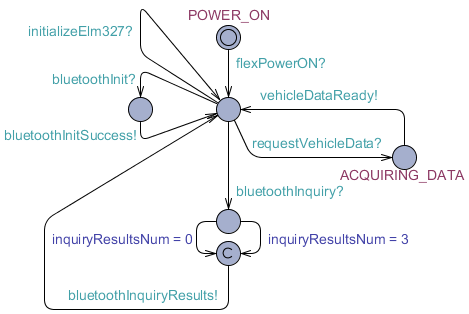
\includegraphics[width=4.7in]{img/FLEX-OBD-LCD_bluetooth}
  \caption{\textit{Bluetooth}}
\end{figure}

As the picture shows, the Bluetooth module wakes up and simply replies to the requests.

In case of inquiry request, nondeterministically returns 0 or 3, simulating the cases in which 0 or 3 devices have been discovered during the inquiry.

\subsection{FLEX-OBD-LCD (standalone)}

In this case, the active parts are:

\begin{itemize}
	\item user: human who pushes buttons and reads the LCD;
	\item bluetooth: Bluetooth module, which also abstracts the Elm327 and the vehicle;
	\item scheduler: tasks manager;
	\item taskMain: task which initializes all the environment and, in the end, activates the other tasks;
	\item taskReceive: task which retrieves vehicle data;
	\item taskUpdateLCD: task which updates the LCD with the data proveded by the taskReceive task.
\end{itemize}

\begin{figure}[H]
  \centering
  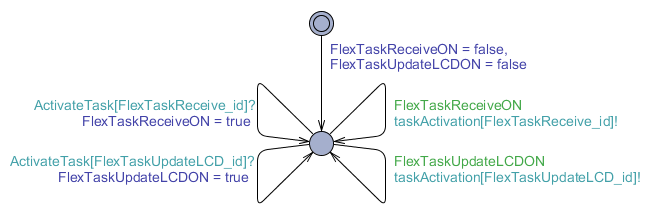
\includegraphics[width=6in]{img/FLEX-OBD-LCD_scheduler}
  \caption{\textit{Scheduler}}
\end{figure}

The scheduler is not the real scheduler. It simply provides a minimal concurrency management between taskUpdateLCD and taskReceive tasks after their activations.

These tasks are activated by the taskMain.

\begin{figure}[H]
  \centering
  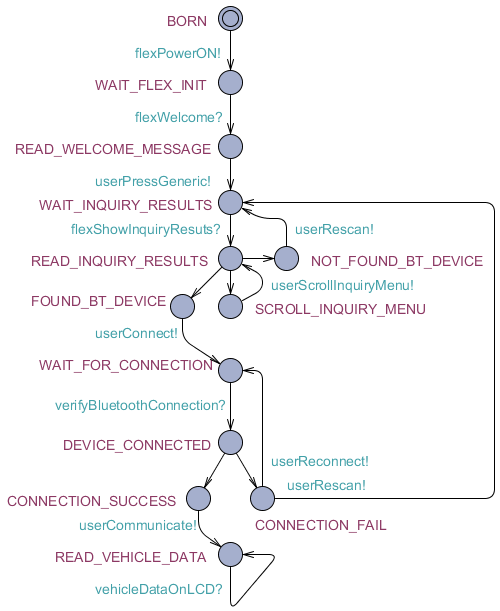
\includegraphics[width=4.7in]{img/FLEX-OBD-LCD_user}
  \caption{\textit{User}}
\end{figure}

User's first action is to power-up the Flex.

After the Flex initialization, the user has to push a button.

After the Flex returned the inquiry results, the user can scroll the inquiry menu, request another inquiry scan or connect to a specific device.

If the user requested the connection, he must also check if the connection has been correctly established (on the Bluetooth module the red led should stop blinking and green led should be turned on).

If the connection failed, then the user can perform another inquiry or retry the connection.

If the connection succeded, then it is possible to start the vehicle communication and the user will be able to read the vehicle data on the LCD screen.

\begin{figure}[H]
  \centering
  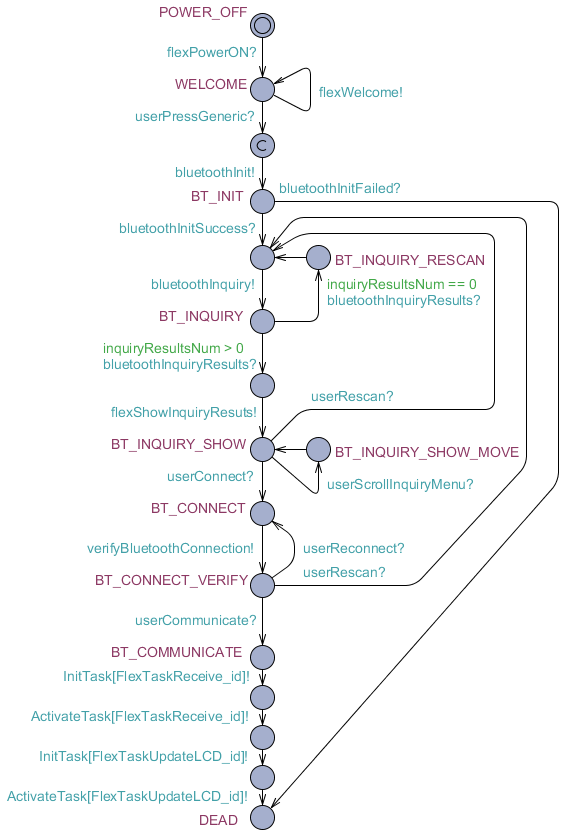
\includegraphics[width=5.7in]{img/FLEX-OBD-LCD_taskMain}
  \caption{\textit{taskMain}}
\end{figure}

The taskMain is the first task to be executed.

First of all, it shows a welcome message on LCD and waits an human response.

After the human response, the Bluetooth module is configured. If the configuration goes wrong, then the task dies and the whole system becomes idle. Otherwise, an inquiry scan is performed.

Inquiry goes on until at least one Bluetooth device is found, then the scan results are shown to the user through a dynamic menu.

User can navigate the menu and decide if perform another inquiry or connect to one of the devices.

After the connection attempt, is requested to the user what to do next, in case of connection success or failure: perform another inquiry, retry to connect, or start the vehicle data transfert.

If the data transfert began, then the other two tasks are initialized and activated.

\begin{figure}[H]
  \centering
  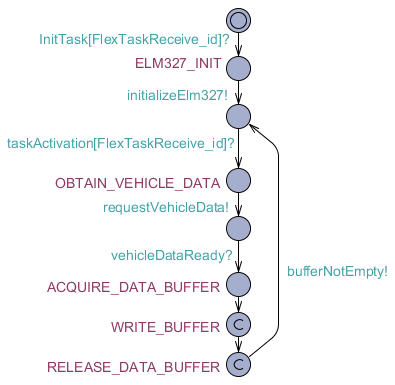
\includegraphics[width=4in]{img/FLEX-OBD-LCD_taskReceive}
  \caption{\textit{taskReceive}}
\end{figure}

The taskReceive is waken up by the taskMain.

It's first operation is to initialize the Elm327, then, periodically, it performs the operations described next.

It request the vehicle new data.

It locks the mutex associated to the shared buffer which contains the vehicle data.

It fills the buffer with new data.

It unlocks the mutex.

It notifies the taskUpdateLCD that new data is ready.

It dies, waiting for next activation to be performed by the scheduler.

\begin{figure}[H]
  \centering
  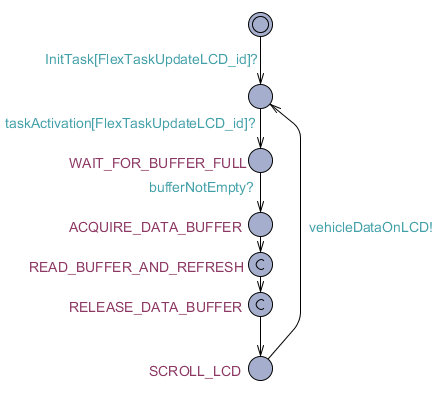
\includegraphics[width=4.5in]{img/FLEX-OBD-LCD_taskUpdateLCD}
  \caption{\textit{taskUpdateLCD}}
\end{figure}

The taskUpdateLCD periodically performs the operations described next.

It waits until the vehicle data buffer contains new data.

It locks the mutex associated with the shared vehicle data buffer.

It locally copies data from the shared buffer.

It releases the mutex.

It checks if the user requested a scroll and shows the data on LCD.

It dies, waiting for next activation to be performed by the scheduler.

%------------------------------------------------\\

\subsection{FLEX-OBD and PC GUI}

In this other case, the active parts are:

\begin{itemize}
	\item PC: system that comprehends the human and the PC program which interacts with the Flex Light;
	\item bluetooth: Bluetooth module, which also abstracts the Elm327 and the vehicle;
	\item scheduler: tasks manager;
	\item taskMain: task which initializes all the environment and, in the end, activates the other tasks;
	\item taskGetData: task which retrieves vehicle data;
	\item taskSendData: task which forwards to the PC the data provided by the taskGetData task.
\end{itemize}

\begin{figure}[H]
  \centering
  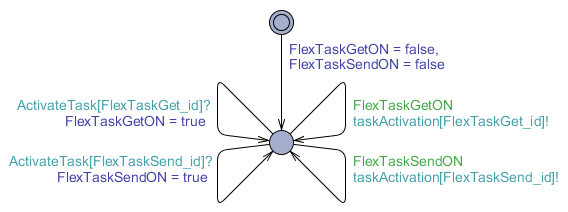
\includegraphics[width=6in]{img/FLEX-PC_scheduler}
  \caption{\textit{Scheduler}}
\end{figure}

The scheduler is not the real scheduler. It simply provides a minimal concurrency management between taskGetData and taskSendData tasks after their activations.

These tasks are activated by the taskMain.

\begin{figure}[H]
  \centering
  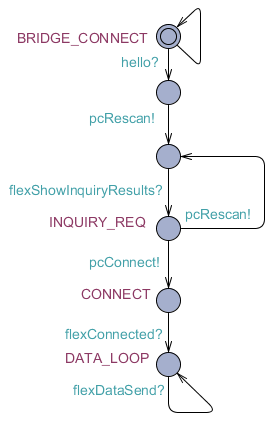
\includegraphics[width=2.7in]{img/FLEX-PC_PC}
  \caption{\textit{PC}}
\end{figure}

The PC loops until the user requests to ping the Flex.

After the ping, the PC has to request an inquiry scan to the Flex.

Once the inquiry results have been received, the PC can reject them, requesting another inquiry, or accept one of them, asking the Flex to establish the connection.

After the Flex confirms that the connection has been succesfully performed, then the PC enters in a loop, receiving and showing vehicle data provided by the Flex.

\begin{figure}[H]
  \centering
  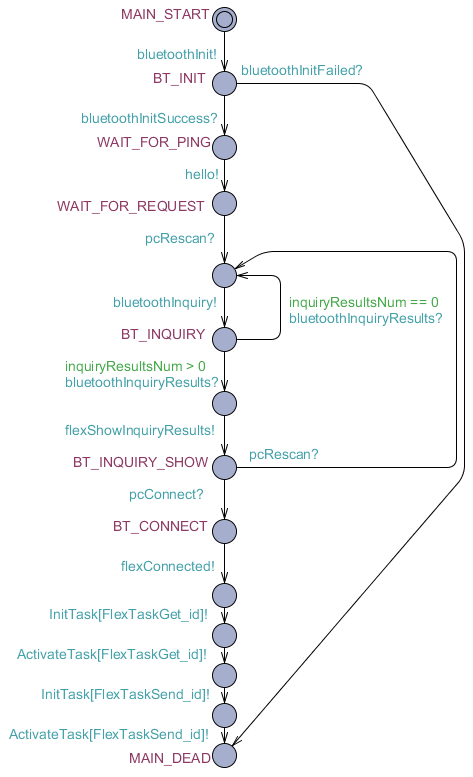
\includegraphics[width=5in]{img/FLEX-PC_taskMain}
  \caption{\textit{taskMain}}
\end{figure}

This task automatically performs the following operations.

It initializes Bluetooth module. If initializzation fails, then this task dies, causing the whole system to become idle. Otherwise, it can wait for the PC ping.

After the PC ping, it waits for the PC to request an inquiry, so it cyclically performs inquiry scans until at least one Bluetooth device is found.

The inquiry results are sent to the PC, which can request another inquiry or can ask to connect to one of the devices discovered by the last scan.

After the connection, this task initializes and activates the taskGetData and taskSendData tasks and dies.

\begin{figure}[H]
  \centering
  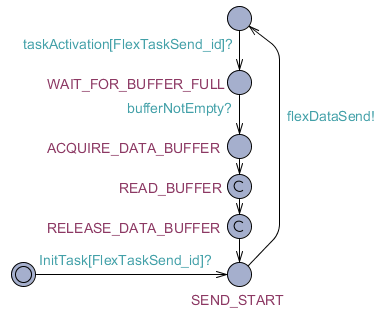
\includegraphics[width=4in]{img/FLEX-PC_taskSendData}
  \caption{\textit{taskSendData}}
\end{figure}

This task periodically performs the operations described next.

It waits for new vehicle data.

It acquires the mutex associated to the shared vehicle data buffer.

It puts the vehicle data buffer contents to local variables.

It releases the mutex.

It sends the new vehicle data to the PC.

It dies, waiting for next activation.

\begin{figure}[H]
  \centering
  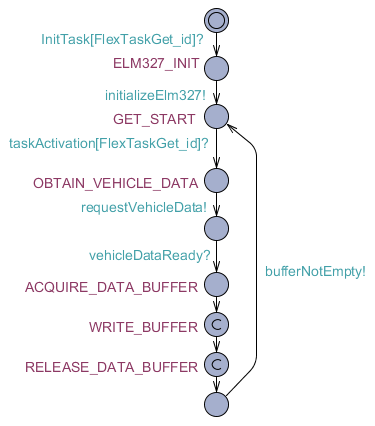
\includegraphics[width=4in]{img/FLEX-PC_taskGetData}
  \caption{\textit{taskGetData}}
\end{figure}

First of all this task initializes the Elm327.

After that, periodically performs the operations described next.

It queries the vehicle to receive new data and locally stores this data.

It locks the mutex associated to the shared vehicle data buffer.

It fills the shared vehicle data buffer with the new data.

It releases the mutex.

It notifies the taskReceive that new data is available and dies, waiting for next activation.

\end{document}